%!TEX root = ../../thesis.tex
\chapter{The Surface Second-Harmonic Generation Yield}\label{chap:sshgyield}
\partialtoc

In Chapter \ref{chap:chi2} we derived the expressions for the nonlinear surface
susceptibility tensor including three features not previously found in a single
formulation: (i) the scissors correction, (ii) the contribution of the nonlocal
part of the pseudopotentials, and (iii) the cut function used to extract the
surface response, all within the independent particle approximation. There are,
of course, several other theoretical formalisms that describe the SHG process
for surfaces with different approximations and varying levels of difficulty
\cite{levinePRB94, mendozaPRL98, arzatePRB01, mendozaPRB01, mejiaPRB02,
sanoPRB02, mejiaRMF04, trollePRB14}. However, I consider that this newly
developed framwork, with the inclusion of these three contributions opens the
possibility to study SSHG with more versatility and accuracy than was previously
available at this level of approximation.

In this chapter, I will walk the reader through the considerations for
developing the three layer (3-layer) model for the SSHG yield, that considers
that the SH conversion takes place in a thin layer just below the surface that
lies under the vacuum region and above the bulk of the material. We will then
derive explicit expressions for each of the four polarization configurations for
the incoming and outgoing fields. These expressions will be simplified by taking
into account the symmetry relations for the (111), (110), and (001) surfaces. I
have also included Appendix \ref{app:sshg_explicit_expressions_rif} that
contains a wealth of supplementary derivations for all the work contained in
this chapter.


%%%%%%%%%%%%%%%%%%%%%%%%%%%%%%%%%%%%%%%%%%%%%%%%%%%%%%%%%%%%%%%%%%%%%%%%%%%%%%%%
%%%%%%%%%%%%%%%%%%%%%%%%%%%%%%%%%%%%%%%%%%%%%%%%%%%%%%%%%%%%%%%%%%%%%%%%%%%%%%%%

\section{The Three Layer Model for the SSHG Yield}\label{sec:3layersshg}

In this section, we will derive the formulas required for the calculation of the
SSHG yield, defined by
\begin{equation}\label{eq:rintensities}
\mathcal{R}(\omega)=\frac{I(2\omega)}{I^2(\omega)},
\end{equation}
with the intensity given by \cite{boyd, sutherland}
\begin{equation}\label{eq:intensity}
I(\omega)=
\left\{
\begin{array}{cc}
\frac{c}{2\pi}n(\omega)|E(\omega)|^{2} & \text{(CGS units)} \\\\
2\epsilon_{0}c\, n(\omega)|E(\omega)|^{2} & \text{(MKS units)}
\end{array}
\right.,
\end{equation}
where $n(\omega)=\sqrt{\epsilon(\omega)}$ is the index of refraction with
$\epsilon(\omega)$ as the dielectric function, $\epsilon_{0}$ is the vacuum
permittivity, and $c$ the speed of light in vacuum.

There are several ways to calculate $R$, one of which is the procedure followed
by Cini \cite{ciniPRB91}. This approach calculates the nonlinear susceptibility
and at the same time the radiated fields. However, I present an alternative
derivation based on the work of Mizrahi and Sipe \cite{mizrahiJOSA88}, since the
derivation of the 3-layer model is straightforward. In this scheme, the surface
is represented by three regions or layers. The first layer is the vacuum region
(denoted by $v$) with a dielectric function $\epsilon_{v}(\omega)=1$ from where
the fundamental electric field $\mathbf{E}_{v}(\omega)$ impinges on the
material. The second layer is a thin layer (denoted by $\ell$) of thickness $d$
characterized by a dielectric function $\epsilon_{\ell}(\omega)$. It is in this
layer where the SHG takes place. The third layer is the bulk region denoted by
$b$ and characterized by $\epsilon_{b}(\omega)$. Both the vacuum and bulk layers
are semi-infinite (see Fig. \ref{fig:MR3layer2w}).

To model the electromagnetic response of the 3-layer model, we follow Ref.
\cite{mizrahiJOSA88} and assume a polarization sheet of the form
\begin{equation}\label{eq:psheet}
\mathbf{P}(\mathbf{r},t) = \boldsymbol{\mathcal{P}}
e^{i\boldsymbol{\kappa}\cdot\mathbf{R}}e^{-i\omega t}\delta(z - z_{\beta}) 
+ \mathrm{c.c.},
\end{equation}
where $\mathbf{R}=(x,y)$, $\boldsymbol{\kappa}$ is the component of the wave
vector $\boldsymbol{\nu}^{\phantom{a}}_{\beta}$ parallel to the surface, and
$z_{\beta}$ is the position of the sheet within medium $\beta$, and
$\boldsymbol{\mathcal{P}}$ is the position independent polarization. Ref.
\cite{sipeJOSAB87} demonstrates that the solution of the Maxwell equations for
the radiated fields $E_{\beta,p\pm}$, and $E_{\beta,s}$ with
$\mathbf{P}(\mathbf{r},t)$ as a source at points $z\neq 0$, can be written as
\begin{equation}\label{eq:solmaxwell}
(E_{\beta,p\pm},E_{\beta,s}) = 
(\frac{\gamma i\tilde{\omega}^2}{\tilde{w}_{\beta}}
\,\hat{\mathbf{p}}_{\beta\pm}\cdot\boldsymbol{\mathcal{P}},
\frac{\gamma i\tilde{\omega}^2}{\tilde{w}_{\beta}}
\,\hat{\mathbf{s}}\cdot\boldsymbol{\mathcal{P}}),
\end{equation} 
where $\gamma=2\pi$ in CGS units or $\gamma=1/2\epsilon_{0}$ in MKS units, and
$\tilde{\omega}=\omega/c$. Also, $\hat{\mathbf{s}}$ and
$\hat{\mathbf{p}}_{\beta\pm}$ are the unitary vectors for the $s$ and $p$
polarizations of the radiated field, respectively. The $\pm$ refers to upward
($+$) or downward ($-$) direction of propagation within medium $\beta$, as shown
in Fig. \ref{fig:MR3layer2w}. Also,
$\tilde{w}^{\phantom{a}}_{\beta}(\omega)=\tilde{\omega}w^{\phantom{a}}_{\beta}$,
where
\begin{equation}\label{eq:r4}
\hat{\mathbf{p}}^{\phantom{A}}_{\beta\pm}(\omega) =
  \frac{\kappa(\omega)\hat{\mathbf{z}}\mp 
  \tilde{w}^{\phantom{A}}_{\beta}(\omega)\hat{\boldsymbol{\kappa}}} 
  {\tilde{\omega} n^{\phantom{A}}_{\beta}(\omega)}
= \frac{\sin\theta_{0}\hat{\mathbf{z}}\mp 
  w^{\phantom{A}}_{\beta}(\omega)\hat{\boldsymbol{\kappa}}} 
  {n^{\phantom{A}}_{\beta}(\omega)},
\end{equation}
with
\begin{equation}\label{eq:wavevector}
w^{\phantom{a}}_{\beta}(\omega) = 
\big(\epsilon^{\phantom{a}}_{\beta}(\omega) - \sin^{2}\theta_{0}\big)^{1/2},
\end{equation}
$\theta_{0}$ is the angle of incidence of $\mathbf{E}_{v}(\omega)$,
$\kappa(\omega)=\vert\boldsymbol{\kappa}\vert = \tilde{\omega}\sin\theta_{0}$,
$n^{\phantom{A}}_{\beta}(\omega)=\sqrt{\epsilon^{\phantom{A}}_{\beta}(\omega)}$
is the index of refraction of medium $\beta$, and $z$ is the direction
perpendicular to the surface that points towards the vacuum. If we consider the
plane of incidence along the $\boldsymbol{\kappa}z$ plane, then
\begin{equation}\label{eq:mc1}
\hat{\boldsymbol{\kappa}} = \cos\phi\hat{\mathbf{x}} + \sin\phi\hat{\mathbf{y}},
\end{equation}
and
\begin{equation}\label{eq:mmc2}
\hat{\mathbf{s}} = -\sin\phi\hat{\mathbf{x}} + \cos\phi\hat{\mathbf{y}},
\end{equation}
where $\phi$ is the azimuthal angle with respect to the $x$ axis.

In the 3-layer model the nonlinear polarization responsible for the SHG is
immersed in the thin layer ($\beta=\ell$), and is given by
\begin{equation}\label{eq:tres}
\mathcal{P}_{\ell,i}(2\omega)=
\left\{
\begin{array}{cc}
\chi^{\mathrm{abc}}_{\mathrm{surface}}(-2\omega;\omega,\omega)
    E^{\mathrm{b}}(\omega)E^{\mathrm{c}}(\omega)
    & \text{(CGS units)}\\\\
\epsilon_{0}\chi^{\mathrm{abc}}_{\mathrm{surface}}(-2\omega;\omega,\omega)
    E^{\mathrm{b}}(\omega)E^{\mathrm{c}}(\omega)
    & \text{(MKS units)}
\end{array}
\right.,
\end{equation}
where $\boldsymbol{\chi}_{\mathrm{surface}}(-2\omega;\omega,\omega)$ is the
dipolar surface nonlinear susceptibility tensor that we derived in Chapter
\ref{chap:chi2}, and the Cartesian indices $\mathrm{a,b,c}$ are summed over if
repeated. As we mentioned before, $\chi^{\mathrm{abc}}(-2\omega;\omega,\omega) =
\chi^{\mathrm{acb}}(-2\omega;\omega,\omega)$ is the intrinsic permutation
symmetry due to the fact that SHG is degenerate in $E_{j}(\omega)$ and
$E_{k}(\omega)$. As in Ref. \cite{mizrahiJOSA88}, we consider the polarization
sheet (Eq. \eqref{eq:psheet}) to be oscillating at some frequency $\omega$ in
order to properly express Eqs. \eqref{eq:solmaxwell}-\eqref{eq:mmc2}. However,
in the following we find it convenient to use $\omega$ exclusively to denote the
fundamental frequency and $\boldsymbol{\kappa}$ to denote the component of the
incident wave vector parallel to the surface. The generated nonlinear
polarization is oscillating at $\Omega = 2\omega$ and will be characterized by a
wave vector parallel to the surface $\mathbf{K} = 2\boldsymbol{\kappa}$. We can
carry over Eqs. \eqref{eq:psheet}-\eqref{eq:mmc2} simply by replacing the
lowercase symbols
($\omega,\tilde{\omega},\boldsymbol{\kappa},n^{\phantom{A}}_{\beta},
\tilde{w}^{\phantom{A}}_{\beta},w^{\phantom{A}}_{\beta},
\hat{\mathbf{p}}^{\phantom{A}}_{\beta\pm},\hat{\mathbf{s}}$) with uppercase
symbols ($\Omega,\tilde{\Omega},\mathbf{K},N^{\phantom{A}}_{\beta},
\tilde{W}^{\phantom{A}}_{\beta},W^{\phantom{A}}_{\beta},
\hat{\mathbf{P}}_{\beta\pm},\hat{\mathbf{S}}$), all evaluated at $2\omega$. Of
course, we always have that $\hat{\mathbf{S}}=\hat{\mathbf{s}}$.

\begin{figure}[t]
\centering 
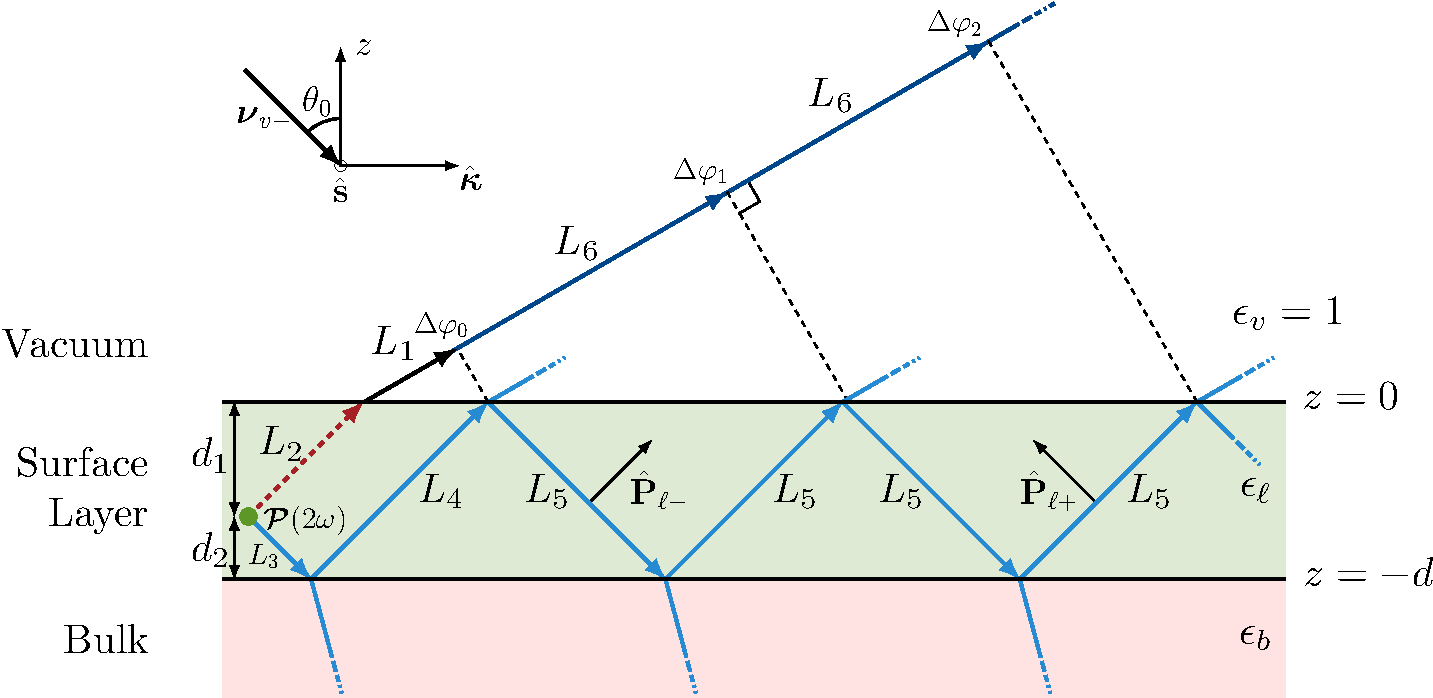
\includegraphics[scale=0.5]{content/figures/diag-3layer_MR_2w}
\caption[Sketch of the three layer model for SHG.]
{Sketch of the three layer model for SHG. The vacuum region ($v$) is on
top with $\epsilon_{v}=1$; the layer $\ell$ of thickness $d = d_{1} + d_{2}$, is
characterized with $\epsilon_{\ell}(\omega)$, and it is where the SH
polarization sheet $\boldsymbol{\mathcal{P}}_{\ell}(2\omega)$ is located at
$z_{\ell} = d_{1}$. The bulk $b$ is described with $\epsilon_{b}(\omega)$. The
arrows point along the direction of propagation, and the $p$-polarization unit
vector, $\hat{\mathbf{P}}_{\ell -(+)}$, along the downward (upward) direction is
denoted with a thick arrow. The $s$-polarization unit vector $\hat{\mathbf{s}}$,
points out of the page. The fundamental field $\mathbf{E}(\omega)$ is incident
from the vacuum side along the $\boldsymbol{\kappa}\hat{z}$-plane, with
$\theta_{0}$ its angle of incidence and $\boldsymbol{\nu}_{v-}$ its wave vector.
$\Delta\varphi_{i}$ denotes the phase difference between the multiple reflected
beams and the first layer-vacuum transmitted beam, denoted by the dashed-red
arrow (of length $L_{2}$) followed by the solid black arrow (of length $L_{1}$).
The dotted lines in the vacuum region are perpendicular to the beam extended
from the solid black arrow (denoted by solid blue arrows of length $L_{6}$).}
\label{fig:MR3layer2w}
\end{figure}

From Fig. \ref{fig:MR3layer2w}, we observe the propagation of the SH field as it
is refracted at the layer-vacuum interface ($\ell v$), and  reflected multiple
times from the layer-bulk ($\ell b$) and layer-vacuum ($\ell v$) interfaces.
Thus, we can define
\begin{equation}\label{eq:r5}
\mathbf{T}^{\ell v}
= \hat{\mathbf{s}}T_{s}^{\ell v}\hat{\mathbf{s}} 
+ \hat{\mathbf{P}}_{v+}T_{p}^{\ell v} \hat{\mathbf{P}}_{\ell +},
\end{equation}
as the transmission tensor for the $\ell v$ interface,
\begin{equation}\label{eq:r6}
\mathbf{R}^{\ell b}
= \hat{\mathbf{s}}R_{s}^{\ell b}\hat{\mathbf{s}}
+ \hat{\mathbf{P}}_{\ell +}R_{p}^{\ell b} \hat{\mathbf{P}}_{\ell -},
\end{equation} 
as the reflection tensor for the $\ell b$ interface, and
\begin{equation}\label{eq:r6b}
\mathbf{R}^{\ell v}
= \hat{\mathbf{s}}R_{s}^{\ell v}\hat{\mathbf{s}}
+ \hat{\mathbf{P}}_{\ell -}R_{p}^{\ell v} \hat{\mathbf{P}}_{\ell +},
\end{equation} 
as the reflection tensor for the $\ell v$ interface. The Fresnel factors in
uppercase letters, $T^{ij}_{s,p}$ and $R^{ij}_{s,p}$, are evaluated at $2\omega$
from the following well known formulas \cite{jacksonbook}
\begin{equation}\label{eq:e.f1}
\begin{split}
t_{s}^{ij}(\omega) &=
\frac{2w_{i}(\omega)}{w_{i}(\omega) + w_{j}(\omega)},
\quad\quad  
t_{p}^{ij}(\omega) =
\frac{2w_{i}(\omega)\sqrt{\epsilon_{i}(\omega)\epsilon_j(\omega)}}
     {w_{i}(\omega)\epsilon_{j}(\omega) + w_{j}(\omega)\epsilon_{i}(\omega)},\\
r_{s}^{ij}(\omega) &=
\frac{w_{i}(\omega) - w_{j}(\omega)}
     {w_{i}(\omega) + w_{j}(\omega)},
\quad\quad 
r_{p}^{ij}(\omega) =
\frac{w_{i}(\omega)\epsilon_{j}(\omega) - w_{j}\epsilon_{i}(\omega)}
     {w_{i}(\omega)\epsilon_{j}(\omega) + w_{j}(\omega)\epsilon_{i}(\omega)}. 
\end{split}
\end{equation}
With these expressions we easily derive the following useful relations,
\begin{equation}\label{eq:mf}
\begin{split}
1 + r^{\ell b}_{s} &= t^{\ell b}_{s},\\
1 + r^{\ell b}_{p} &= \frac{n_{b}}{n_{\ell}}t^{\ell b}_{p},\\
1 - r^{\ell b}_{p} &= \frac{n_{\ell}}{n_{b}}\frac{w_{b}}{w_{\ell}}
                      t^{\ell b}_{p},\\
t^{\ell v}_{p} &= \frac{w_{\ell}}{w_{v}}t^{v\ell}_{p},\\
t^{\ell v}_{s} &= \frac{w_{\ell}}{w_{v}}t^{v\ell}_{s}.
\end{split}
\end{equation}


%%%%%%%%%%%%%%%%%%%%%%%%%%%%%%%%%%%%%%%%%%%%%%%%%%%%%%%%%%%%%%%%%%%%%%%%%%%%%%%%

\subsection{Multiple SHG reflections}

The SH field $\mathbf{E}(2\omega)$ radiated by the SH polarization
$\boldsymbol{\mathcal{P}}_{\ell}(2\omega)$ will radiate directly into the vacuum
and the bulk, where it will be reflected back at the layer-bulk interface into
the thin layer. This beam will be transmitted and reflected multiple times, as
shown in Fig. \ref{fig:MR3layer2w}. As the two beams propagate, a phase
difference will develop between them according to
\begin{equation}\label{eq:m99}
\begin{split}
\Delta\varphi_{m} 
&= \tilde{\Omega}
\Big(
(L_{3} + L_{4} + 2mL_{5})N_{\ell}
 - \big(L_{2}N_{\ell} + (L_{1} + mL_{6})N_{v}\big)
\Big)\\
&= \delta_{0} + m\delta\quad m=0,1,2,\ldots,
\end{split}
\end{equation}
where
\begin{equation}\label{eq:delta0}
\delta_{0} =
8\pi\left(\frac{d_{2}}{\lambda_{0}}\right)W_{\ell},
\end{equation}
and
\begin{equation}\label{eq:delta}
\delta = 8\pi
\left(\frac{d}{\lambda_{0}}\right)W_{\ell},
\end{equation}
where $\lambda_{0}$ is the wavelength of the fundamental field in the vacuum,
$d$ is the thickness of layer $\ell$, and $d_{2}$ is the distance of
$\boldsymbol{\mathcal{P}}_{\ell}(2\omega)$ from the $\ell b$ interface (see Fig.
\ref{fig:MR3layer2w}). We see that $\delta_{0}$ is the phase difference of the
first and second transmitted beams, and $m\delta$ that of the first and third
($m = 1$), first and fourth ($m = 2$), and so on. Note that the thickness $d$ of
the layer $\ell$ enters through the phase $\delta$, and the position $d_{2}$ of
the nonlinear polarization sheet $\mathbf{P}(\mathbf{r},t)$ (Eq.
\eqref{eq:psheet}) enters through $\delta_{0}$. In particular, $d_{2}$ could be
used as a variable to study the effects of multiple reflections on the SSHG
yield $\mathcal{R}(2\omega)$.

To take into account the multiple reflections of the generated SH field in the
layer $\ell$, we proceed as follows. I include the algebra for the $p$-polarized
SH field, and the $s$-polarized field could be worked out along the same steps.
The $p$-polarized $\mathbf{E}_{\ell,p}(2\omega)$ field reflected multiple times
is given by
\begin{equation}\label{eq:E2wcomplete}
\begin{split}
\mathbf{E}_{\ell,p}(2\omega) 
&= E_{\ell,p+}(2\omega)\mathbf{T}^{\ell v}\cdot\hat{\mathbf{P}}_{\ell +}
 + E_{\ell,p-}(2\omega)\mathbf{T}^{\ell v}
\cdot\mathbf{R}^{\ell b}\cdot\hat{\mathbf{P}}_{\ell-}e^{i\Delta\varphi_{0}}\\
&+ E_{\ell,p-}(2\omega)\mathbf{T}^{\ell v}
\cdot\mathbf{R}^{\ell b}\cdot\mathbf{R}^{\ell v}
\cdot\mathbf{R}^{\ell b}\cdot\hat{\mathbf{P}}_{\ell-}e^{i\Delta\varphi_{1}}
\\
&+ E_{\ell,p-}(2\omega)\mathbf{T}^{\ell v}
\cdot\mathbf{R}^{\ell b}\cdot\mathbf{R}^{\ell v}
\cdot\mathbf{R}^{\ell b}\cdot\mathbf{R}^{\ell v}
\cdot\mathbf{R}^{\ell b}\cdot\hat{\mathbf{P}}_{\ell-}e^{i\Delta\varphi_{2}}
+\cdots\\
&= E_{\ell,p+}(2\omega)\mathbf{T}^{\ell v}\cdot\hat{\mathbf{P}}_{\ell +}
+ E_{\ell,p-}(2\omega) \mathbf{T}^{\ell v}
\cdot\sum_{m=0}^\infty  
\big(
\mathbf{R}^{\ell b}\cdot\mathbf{R}^{\ell v} 
e^{i\delta}\Big)^m 
\cdot\mathbf{R}^{\ell b}\cdot\hat{\mathbf{P}}_{\ell-}e^{i\delta_{0}}.
\end{split}
\end{equation}
From Eqs. \eqref{eq:r5} - \eqref{eq:r6b} it is easy to show that
\begin{equation*}\label{eq:m1}
\mathbf{T}^{\ell v}\cdot
\Big(\mathbf{R}^{\ell b}\cdot\mathbf{R}^{\ell v}\Big)^{n}\cdot
\mathbf{R}^{\ell b}
= \hat{\mathbf{s}}T^{\ell v}_{s}
  \Big(R^{\ell b}_{s}R^{\ell v}_{s}\Big)^{n}R^{\ell b}_{s}\hat{\mathbf{s}}
+ \hat{\mathbf{P}}_{v+}T^{\ell v}_{p}\Big(R^{\ell b}_{p}R^{\ell v}_{p}\Big)^n 
  R^{\ell b}_{p} 
\hat{\mathbf{P}}_{\ell-},
\end{equation*}
then,
\begin{equation}\label{eq:E2wreduced}
\mathbf{E}_{\ell,p}(2\omega) 
= \hat{\mathbf{P}}_{\ell +}T^{\ell v}_{p}
\Big(
E_{\ell,p+}(2\omega) +
\frac{R^{\ell b}_{p}e^{i\delta_{0}}}{1 + R^{v\ell}_{p}R^{\ell b}_{p}e^{i\delta}}
E_{\ell,p-}(2\omega) 
\Big),
\end{equation}
where we used $R^{ij}_{s,p} = -R^{ji}_{s,p}$. Using Eq. \eqref{eq:solmaxwell}
and \eqref{eq:mf}, we can readily write
\begin{equation}\label{eq:mr8}
\mathbf{E}_{\ell,p}(2\omega) =
\frac{\gamma i\tilde{\Omega}}{W_{\ell}}\mathbf{H}_{\ell}\cdot
\boldsymbol{\mathcal{P}}_{\ell}(2\omega),
\end{equation}
where
\begin{equation}\label{eq:mr9}
\mathbf{H}_{\ell}
= \frac{W_\ell}{W_v}
\left[
\hat{\mathbf{s}}\,T_{s}^{v\ell}
\left(1+ R^{M}_{s}\right)\hat{\mathbf{s}} + \hat{\mathbf{P}}_{v+}T_{p}^{v\ell}
\left(\hat{\mathbf{P}}_{\ell +} + R^{M}_{p}\hat{\mathbf{P}}_{\ell -}\right)
\right],
\end{equation}
and
\begin{equation}\label{m61}
R^{M}_{\mathrm{i}}\equiv
\frac{R^{\ell b}_{\mathrm{i}}e^{i\delta_{0}}}
     {1+R^{v\ell}_{\mathrm{i}} R^{\ell b}_{\mathrm{i}}e^{i\delta}},
     \quad \mathrm{i}=s,p,
\end{equation}
is defined as the multiple ($M$) reflection coefficient. This coefficient
depends on the thickness $d$ of layer $\ell$, and most importantly on the
position $d_{2}$ of $\boldsymbol{\mathcal{P}}_{\ell}(2\omega)$ within this
layer. The final results will depend on both $d$ and $d_{2}$. However, using Eq.
\eqref{eq:delta0} we can also define an average $\bar{R}^{M}_{\mathrm{i}}$ as
\begin{equation}\label{eq:mcave}
\bar{R}^{M}_{\mathrm{i}}\equiv 
\frac{1}{d}\int_{0}^{d}
\frac{R^{\ell b}_{\mathrm{i}}e^{i(8\pi W_{\ell}/\lambda_{0})x}}
{1 + R^{v\ell}_{\mathrm{i}}R^{\ell b}_{\mathrm{i}}e^{i\delta}}\,dx
= \frac{R^{\ell b}_{\mathrm{i}}e^{i\delta/2}}
{1 + R^{v\ell}_{\mathrm{i}}R^{\ell b}_{\mathrm{i}}e^{i\delta}}
\,\mathrm{sinc}(\delta/2),
\end{equation}
that only depends on $d$ through the $\delta$ term from Eq. \eqref{eq:delta}.

To connect with the work in Ref. \cite{mizrahiJOSA88}, where
$\boldsymbol{\mathcal{P}}(2\omega)$ is located on top of the vacuum-surface
interface and only the vacuum radiated beam and the first (and only) reflected
beam need be considered, we take $\ell = v$ and $d_{2} = 0$, then $T^{\ell v} =
1$, $R^{v\ell} = 0$ and $\delta_{0} = 0$, with which $R^{M}_{\mathrm{i}} =
R^{vb}_{\mathrm{i}}$. Thus, Eq. \eqref{eq:mr9} coincides with Eq. (3.8) of Ref.
\cite{mizrahiJOSA88}.


%%%%%%%%%%%%%%%%%%%%%%%%%%%%%%%%%%%%%%%%%%%%%%%%%%%%%%%%%%%%%%%%%%%%%%%%%%%%%%%%

\subsection{Multiple Reflections for the Linear Field}

For a more complete formulation, we must also consider the multiple reflections
of the fundamental field $\mathbf{E}_{\ell}(\omega)$ inside the thin $\ell$
layer. In Fig. \ref{fig:MR3layer1w} I present the situation where
$\mathbf{E}_{v}(\omega)$ impinges from the vacuum side with an angle of
incidence $\theta_{0}$. As the first transmitted beam is multiply reflected from
the $\ell b$ and the $\ell v$ interfaces, it accumulates a phase difference of
$n\phi$, with $n=1,2,3,\ldots$, given by
\begin{equation}\label{mphi}
\begin{split}
\varphi &= \frac{\omega}{c}(2L_{1}n_{\ell} - L_{2}n_{v})\\
&= 4\pi\left(\frac{d}{\lambda_{0}}\right)w_{\ell},
\end{split}
\end{equation}
where $n_{v}=1$. Besides the equivalent of Eqs. \eqref{eq:r6} and \eqref{eq:r6b}
for $\omega$, we also need
\begin{equation}\label{eq:mvv}
\mathbf{t}^{v\ell}
= \hat{\mathbf{s}}t_{s}^{v\ell}\hat{\mathbf{s}} 
+ \hat{\mathbf{p}}_{\ell -}t_{p}^{v\ell}\hat{\mathbf{p}}_{v-},
\end{equation}
to write
\begin{align}\label{eq:mcvew}
\mathbf{E}(\omega)
&= E_{0}
\Big[
\mathbf{t}^{v\ell} + \mathbf{r}^{\ell b}\cdot\mathbf{t}^{v\ell}e^{i\varphi}
 + \mathbf{r}^{\ell b}\cdot\mathbf{r}^{\ell v}\cdot
   \mathbf{r}^{\ell b}\cdot\mathbf{t}^{v\ell} e^{i2\varphi}
 + \mathbf{r}^{\ell b}\cdot\mathbf{r}^{\ell v}\cdot
   \mathbf{r}^{\ell b}\cdot\mathbf{r}^{\ell v}\cdot
   \mathbf{r}^{\ell b}\cdot\mathbf{t}^{v\ell} e^{i3\varphi}
 + \cdots
\Big]\cdot\hat{\mathbf{e}}^{\mathrm{i}}\nonumber\\
&= E_{0}
\Big[
1 + \Big(1 + \mathbf{r}^{\ell b}\cdot\mathbf{r}^{\ell v}e^{i\varphi}
+ (\mathbf{r}^{\ell b}\cdot\mathbf{r}^{\ell v})^2e^{i2\varphi}+\cdots\Big)\cdot
\mathbf{r}^{\ell b}e^{i\varphi}
\Big]
\cdot\mathbf{t}^{v\ell}\cdot\hat{\mathbf{e}}^{\mathrm{i}}\nonumber\\
&= E_{0}
\Big[
\hat{\mathbf{s}} t^{v\ell}_{s}(1+r^{M}_{s})\hat{\mathbf{s}} 
+ t^{v\ell}_{p}
\left(\hat{\mathbf{p}}_{\ell-}+\hat{\mathbf{p}}_{\ell+}r^{M}_{p}\right)
\hat{\mathbf{p}}_{v-}
\Big]\cdot\hat{\mathbf{e}}^{\mathrm{i}},
\end{align}
where $E_{0}$ is the intensity of the fundamental field, and
$\hat{\mathbf{e}}^{\mathrm{i}}$ is the unit vector of the incoming polarization,
with $\mathrm{i} = s,p$, and then, $\hat{\mathbf{e}}^{s}=\hat{\mathbf{s}}$ and
$\hat{\mathbf{e}}^{p}=\hat{\mathbf{p}}_{v-}$. Also,
\begin{equation}\label{mvrm}
r^{M}_{\mathrm{i}} \equiv
\frac{r^{\ell b}_{\mathrm{i}}e^{i\varphi}}{1+r^{v\ell}_{\mathrm{i}}
r^{\ell b}_{\mathrm{i}}e^{i\varphi}}, \quad \mathrm{i}=s,p.
\end{equation}
$r^{M}_{\mathrm{i}}$ is defined as the multiple (M) reflection coefficient for
the fundamental field. We define $\mathbf{E}^{\mathrm{i}}_{\ell}(\omega)\equiv
E_{0}\mathbf{e}^{\omega,\mathrm{i}}_{\ell}$ ($\mathrm{i}=s,p$), where
\begin{equation}\label{eq:mcvew2}
\mathbf{e}^{\omega,\mathrm{i}}_\ell 
= \Big[\hat{\mathbf{s}} t^{v\ell}_s(1+r^M_s)\hat{\mathbf{s}} 
+ t^{v\ell}_p\left(\hat{\mathbf{p}}_{\ell-}+\hat{\mathbf{p}}_{\ell+}r^{M}_p 
\right)\hat{\mathbf{p}}_{v-}
\Big]\cdot\hat{\mathbf{e}}^{\mathrm{i}},
\end{equation}
and using Eq. \eqref{eq:r4} we obtain that
\begin{equation}\label{eq:mcvep}
\mathbf{e}^{\omega,p}_{\ell}=\frac{t^{v\ell}_{p}}{n_{\ell}}
\left( 
  r^{M+}_{p}\sin\theta_{0}\hat{\mathbf{z}}
+ r^{M-}_{p}w_{\ell}\hat{\boldsymbol{\kappa}}
\right),
\end{equation} 
for $p$-input polarization with
$\hat{\mathbf{e}}^{\mathrm{i}}=\hat{\mathbf{p}}_{v-}$, and
\begin{equation}\label{eq:mcves}
\mathbf{e}^{\omega,s}_\ell=t^{v\ell}_{s}r^{M+}_{s}\hat{\mathbf{s}},
\end{equation}
for $s$-input polarization with
$\hat{\mathbf{e}}^{\mathrm{i}}=\hat{\mathbf{s}}$, where
\begin{equation}\label{eq:mvc}
r^{M\pm}_{\mathrm{i}}=1\pm r^{M}_{\mathrm{i}},\quad \mathrm{i} = s,p.
\end{equation}

\begin{figure}[t]
\centering 
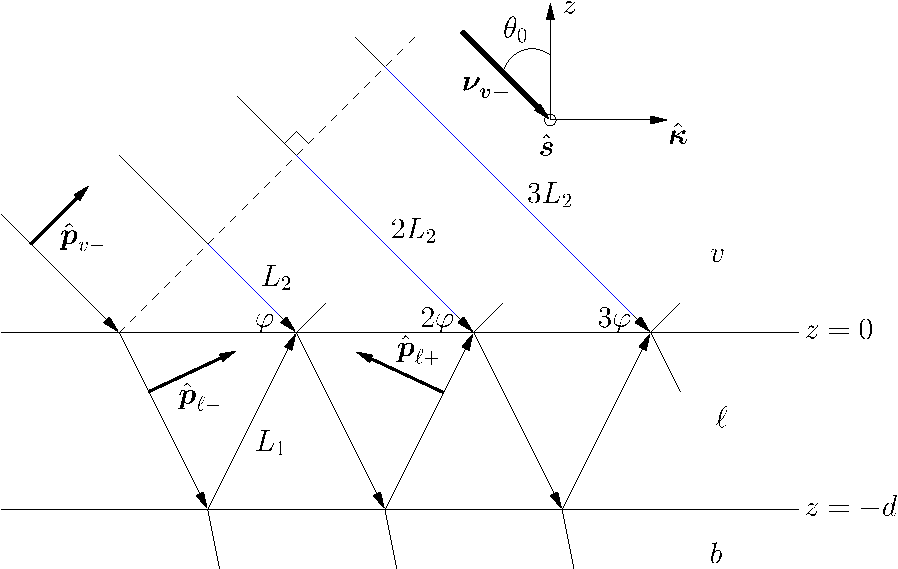
\includegraphics[scale=0.6]{content/figures/diag-3layer_MR_1w}
\caption[Sketch for the multiple reflected, $1\omega$ incoming field.]
{Sketch for the multiple reflected fundamental field
$\mathbf{E}(\omega)$, which impinges from the vacuum side along the
$\hat{\boldsymbol{\kappa}}z$-plane. $\theta_{0}$ and $\boldsymbol{\nu}_{v-}$ are
the angle of incidence and wave vector, respectively. The arrows point along the
direction of propagation. The $p$-polarization unit vectors
$\hat{\mathbf{p}}_{\beta\pm}$, point along the downward $(-)$ or upward $(+)$
directions and are denoted with thick arrows, where $\beta = v$ or $\ell$. The
$s$-polarization unit vector $\hat{\mathbf{s}}$ points out of the page.
$(1,2,3,\ldots)\varphi$ denotes the phase difference for the multiple reflected
beams with respect to the incident field, where the dotted line is perpendicular
to this beam.}
\label{fig:MR3layer1w}
\end{figure}


%%%%%%%%%%%%%%%%%%%%%%%%%%%%%%%%%%%%%%%%%%%%%%%%%%%%%%%%%%%%%%%%%%%%%%%%%%%%%%%%

\subsection{Deriving the SSHG yield}

The magnitude of the radiated field is given by $E(2\omega) =
\hat{\mathbf{e}}^{\mathrm{F}}\cdot\mathbf{E}_{\ell}(2\omega)$, where
$\hat{\mathbf{e}}^{\mathrm{F}}$ is the unit vector of the final, $S$ or $P$ SH
polarization with $\mathrm{F}=S,P$, where $\hat{\mathbf{e}}^S=\hat{\mathbf{s}}$
and $\hat{\mathbf{e}}^P=\hat{\mathbf{P}}_{v+}$. We expand the rightmost term in
parenthesis of Eq. \eqref{eq:mr9} as
\begin{equation}
\begin{split}
\hat{\mathbf{P}}_{\ell +} + R^{M}_{p}\hat{\mathbf{P}}_{\ell -}
&= \frac{\sin\theta_{0}\hat{\mathbf{z}} - W_{\ell}\hat{\boldsymbol{\kappa}}}
        {N_{\ell}}
 + R^{M}_{p}
   \frac{\sin\theta_{0}\hat{\mathbf{z}} + W_{\ell}\hat{\boldsymbol{\kappa}}}
        {N_{\ell}}\\
&= \frac{1}{N_{\ell}}
\left(
\sin\theta_{0}R^{M+}_{p}\hat{\mathbf{z}}
- W_{\ell}R^{M-}_{p}\hat{\boldsymbol{\kappa}}
\right),
\end{split}
\end{equation}
where
\begin{equation}\label{eq:rm}
R^{M\pm}_{\mathrm{i}}\equiv 1 \pm R^{M}_{\mathrm{i}}, \quad \mathrm{i}=s,p.
\end{equation}
Using Eq. \eqref{eq:mf} we write Eq. \eqref{eq:mr8} as
\begin{equation}\label{eq:r10}
E(2\omega) = \frac{2\gamma i\omega}{cW_\ell}
\hat{\mathbf{e}}^{\mathrm{F}}\cdot\mathbf{H}_{\ell}\cdot
\boldsymbol{\mathcal{P}}_{\ell}(2\omega) 
= \frac{2\gamma i\omega}{cW_{v}}
\mathbf{e}^{\,2\omega,\mathrm{F}}_{\ell}\cdot
\boldsymbol{\mathcal{P}}_{\ell}(2\omega),
\end{equation}
where
\begin{equation}\label{eq:r12mm}
\mathbf{e}^{2\omega,\mathrm{F}}_{\ell} =\hat{\mathbf{e}}^{\mathrm{F}}\cdot 
\Bigg[
\hat{\mathbf{s}}T_{s}^{v\ell}R^{M+}_{s}\hat{\mathbf{s}} + 
\hat{\mathbf{P}}_{v+}
\frac{T^{v\ell}_{p}}
     {N_{\ell}}
\left(
\sin\theta_{0}R^{M+}_{p}\hat{\mathbf{z}}
- W_{\ell}R^{M-}_{p}\hat{\boldsymbol{\kappa}}
\right) 
\Bigg]. 
\end{equation}  
Replacing $\mathbf{E}(\omega)\to E_0\mathbf{e}^{\omega,\mathrm{i}}_\ell$, in Eq.
\eqref{eq:tres}, we obtain that
\begin{equation}\label{eq:m4}
\boldsymbol{\mathcal{P}}_{\ell}(2\omega) = 
\left\{
\begin{array}{cc}  
E^{2}_{0}\,
\boldsymbol{\chi}_{\mathrm{surface}}:\mathbf{e}^{\omega,\mathrm{i}}_{\ell}
                  \mathbf{e}^{\omega,\mathrm{i}}_{\ell}
& \text{(CGS units)}\\\\
\epsilon_{0}E^{2}_{0}\,
\boldsymbol{\chi}_{\mathrm{surface}}:\mathbf{e}^{\omega,\mathrm{i}}_{\ell}
                  \mathbf{e}^{\omega,\mathrm{i}}_{\ell}
& \text{(MKS units)}\\
\end{array}
\right.,
\end{equation}
where $\mathbf{e}^{\omega,\mathrm{i}}_{\ell}$ is given by Eq. \eqref{eq:mcvew2},
and thus Eq. \eqref{eq:r10} reduces to ($W_{v}=\cos\theta_{0}$)
\begin{equation}\label{eq:mr10}
E_{\ell}(2\omega) 
= \frac{2\eta i \omega}{c\cos\theta_{0}}
\mathbf{e}^{2\omega,\mathrm{F}}_{\ell}\cdot
\boldsymbol{\chi}_{\mathrm{surface}}:\mathbf{e}^{\omega,\mathrm{i}}_{\ell}
                  \mathbf{e}^{\omega,\mathrm{i}}_{\ell},
\end{equation}
where $\eta=2\pi$ in CGS units and $\eta=1/2$ in MKS units. For ease of
notation, we define
\begin{align}\label{eq:mc0}
\Upsilon_{\mathrm{iF}}
\equiv 
\mathbf{e}^{2\omega,\mathrm{F}}_{\ell}\cdot
\boldsymbol{\chi}_{\mathrm{surface}}:\mathbf{e}^{\omega,\mathrm{i}}_{\ell}
                  \mathbf{e}^{\omega,\mathrm{i}}_{\ell},
\end{align}
where i stands for the incoming polarization of the fundamental electric field
given by $\hat{\mathbf{e}}^{\mathrm{i}}$ in Eq. \eqref{eq:mcvew2}, and F for the
outgoing polarization of the SH electric field given by
$\hat{\mathbf{e}}^{\mathrm{F}}$ in Eq. \eqref{eq:r12mm}. I purposely omitted the
full $\boldsymbol{\chi}(-2\omega;\omega,\omega)$ notation, and will do so from
this point on.

From Eqs. \eqref{eq:rintensities} and \eqref{eq:intensity} we obtain that in
CGS units ($\eta=2\pi$), 
\begin{align}\label{eq:r01}
\vert E(2\omega)\vert^{2} &=
\vert E_{0}\vert^{4}\frac{16\pi^{2}\omega^{2}}{c^{2}W^2_{v}}
\vert\Upsilon_{\mathrm{iF}}\vert^{2}\nonumber\\
%%%%%%%%%%%%%%%%%%%%%%%%%%%%%%%%%%%%%%%%%%%%%%%%%%%%%
\frac{c}{2\pi}\vert\sqrt{N_{v}}E(2\omega)\vert^{2} &=
\frac{32\pi^{3}\omega^{2}}{c^{3}\cos^2\theta_{0}}
\left\vert\frac{\sqrt{N_{v}}}{n^{2}_{\ell}}\Upsilon_{\mathrm{iF}}\right\vert^{2} 
\left(\frac{c}{2\pi}\vert\sqrt{n_{\ell}}E_{0}\vert^{2}\right)^{2}\nonumber\\ 
%%%%%%%%%%%%%%%%%%%%%%%%%%%%%%%%%%%%%%%%%%%%%%%%%%%%%
I(2\omega) &=
\frac{32\pi^{3}\omega^{2}}{c^{3}\cos^2\theta_{0}}
\left\vert\frac{\sqrt{N_{v}}}{n^{2}_{\ell}}\Upsilon_{\mathrm{iF}}\right\vert^{2}
I^{2}(\omega)\nonumber\\
%%%%%%%%%%%%%%%%%%%%%%%%%%%%%%%%%%%%%%%%%%%%%%%%%%%%%
\mathcal{R}_{\mathrm{iF}}(2\omega) &=
\frac{32\pi^{3}\omega^{2}}{c^{3}\cos^2\theta_{0}}
\left\vert\frac{1}{n_{\ell}}\Upsilon_{\mathrm{iF}}\right\vert^{2},
\end{align} 
and in MKS units ($\eta=1/2$),
\begin{align}\label{r01m}
\vert E(2\omega)\vert^{2} &=
\vert E_{0}\vert^{4}\frac{\omega^{2}}{c^{2}W^{2}_{v}}\nonumber\\
%%%%%%%%%%%%%%%%%%%%%%%%%%%%%%%%%%%%%%%%%%%%%%%%%%%%%
2\epsilon_{0}c|\sqrt{N_{v}}E(2\omega)|^{2} &=
\frac{2\epsilon_{0}\omega^{2}}{c\cos^{2}\theta_{0}}
\left\vert\frac{\sqrt{N_{v}}}{n^{2}_{\ell}}\Upsilon_{\mathrm{iF}}\right\vert^{2} 
\frac{1}{4\epsilon^{2}_0c^{2}}
\left(2\epsilon_{0}c\vert\sqrt{n_{\ell}}E_{0}\vert^{2}\right)^{2}\nonumber\\
%%%%%%%%%%%%%%%%%%%%%%%%%%%%%%%%%%%%%%%%%%%%%%%%%%%%%
I(2\omega) &= 
\frac{\omega^{2}}{2\epsilon_{0}c^3\cos^{2}\theta_{0}}
\left\vert\frac{\sqrt{N_{v}}}{n^{2}_{\ell}}\Upsilon_{\mathrm{iF}}\right\vert^{2}
I^{2}(\omega)\nonumber\\
%%%%%%%%%%%%%%%%%%%%%%%%%%%%%%%%%%%%%%%%%%%%%%%%%%%%%
\mathcal{R}_{\mathrm{iF}}(2\omega) &=
\frac{\omega^{2}}{2\epsilon_{0}c^3\cos^{2}\theta_{0}}
\left\vert  \frac{1}{n_{\ell}}\Upsilon_{\mathrm{iF}}\right\vert^{2}.
\end{align}
Finally, we condense these results and establish the SSHG yield as
\begin{equation}\label{eq:mc6}
\mathcal{R}_{\mathrm{iF}}(2\omega) 
\left\{
\begin{array}{ r c } 
\frac{32\pi^{3}\omega^{2}}{c^{3}\cos^{2}\theta_{0}}
\left\vert\frac{1}{n_{\ell}}\Upsilon_{\mathrm{iF}}\right\vert^{2} 
& \text{(CGS units)} \\\\
\frac{\omega^{2}}{2\epsilon_{0}c^3\cos^{2}\theta_{0}}
\left\vert\frac{1}{n_{\ell}}\Upsilon_{\mathrm{iF}}\right\vert^{2} 
& \text{(MKS units)} 
\end{array}
\right.,
\end{equation}
where $N_{v}=1$ and $W_{v}=\cos\theta_{0}$. As mentioned in Chapter
\eqref{chap:chi2}, $\boldsymbol{\chi}_{\mathrm{surface}}$ is given in m$^{2}$/V
in the MKS unit system, since it is a surface second order nonlinear
susceptibility, and $\mathcal{R}_{\mathrm{iF}}$ is given in m$^2$/W.


%%%%%%%%%%%%%%%%%%%%%%%%%%%%%%%%%%%%%%%%%%%%%%%%%%%%%%%%%%%%%%%%%%%%%%%%%%%%%%%%
%%%%%%%%%%%%%%%%%%%%%%%%%%%%%%%%%%%%%%%%%%%%%%%%%%%%%%%%%%%%%%%%%%%%%%%%%%%%%%%%

\section{\texorpdfstring{$\mathcal{R}_{\mathrm{iF}}$}{R} for Different
Polarization Cases}\label{sec:rcases}

We now have everything we need to derive explicit expressions for
$\mathcal{R}_{\mathrm{iF}}$, Eq. \eqref{eq:mc6}, for the most commonly used
polarizations of incoming and outgoing fields (iF=$pP$, $pS$, $sP$, and $sS$).
For this, we must expand $\Upsilon_{\mathrm{iF}}$ from Eq. \eqref{eq:mc0} for
each case. By substituting Eqs. \eqref{eq:mc1} and \eqref{eq:mmc2} into Eq.
\eqref{eq:r12mm}, we obtain
\begin{equation}\label{eq:e2wpmr}
\mathbf{e}^{2\omega,P}_{\ell} =
\frac{T^{v\ell}_{p}}{N_{\ell}}
\big(
  \sin\theta_{0}R^{M+}_{p}\hat{\mathbf{z}}
- W_{\ell}R^{M-}_{p}\cos\phi\hat{\mathbf{x}}
- W_{\ell}R^{M-}_{p}\sin\phi\hat{\mathbf{y}}
\big),
\end{equation}
for $P$ $(\hat{\mathbf{e}}^{\mathrm{F}} = \hat{\mathbf{P}}_{v+})$ outgoing
polarization, and
\begin{equation}\label{eq:e2wsmr}
\mathbf{e}^{2\omega,S}_{\ell} =
T_{s}^{v\ell}R^{M+}_{s}
\left(
- \sin\phi\hat{\mathbf{x}}
+ \cos\phi\hat{\mathbf{y}}
\right).
\end{equation}
for $S$ $(\hat{\mathbf{e}}^{\mathrm{F}}=\hat{\mathbf{s}})$ outgoing
polarization.

Following a similar procedure, we use Eqs. \eqref{eq:mc1} and \eqref{eq:mmc2}
with Eq. \eqref{eq:mcvep}, and obtain
\begin{equation}\label{eq:ewewpmr}
\begin{split}
\mathbf{e}^{\omega,\mathrm{p}}_{\ell}\mathbf{e}^{\omega,\mathrm{p}}_{\ell} =
\left(\frac{t^{v\ell}_{p}}{n_{\ell}}\right)^{2}
\bigg(
  \big(&r^{M-}_{p}\big)^{2}w^{2}_{\ell}\cos^{2}\phi
  \hat{\mathbf{x}}\hat{\mathbf{x}}
+ 2\big(r^{M-}_{p}\big)^{2}w^{2}_{\ell}\sin\phi\cos\phi
  \hat{\mathbf{x}}\hat{\mathbf{y}}\\
+ 2&r^{M+}_{p}r^{M-}_{p}w_{\ell}\sin\theta_{0}\cos\phi
  \hat{\mathbf{x}}\hat{\mathbf{z}}
+ \big(r^{M-}_{p}\big)^{2}w^{2}_{\ell}\sin^{2}\phi
  \hat{\mathbf{y}}\hat{\mathbf{y}}\\
+ 2&r^{M+}_{p}r^{M-}_{p}w_{\ell}\sin\theta_{0}\sin\phi
  \hat{\mathbf{y}}\hat{\mathbf{z}}
+ \big(r^{M+}_{p}\big)^{2}\sin^{2}\theta_{0}
   \hat{\mathbf{z}}\hat{\mathbf{z}}
\bigg),
\end{split}
\end{equation}
for $p$ incoming polarization $(\hat{\mathbf{e}}^{\mathrm{i}} =
\hat{\mathbf{p}}_{v-})$, and with Eq. \eqref{eq:mcves},
\begin{equation}\label{eq:ewewsmr}
\mathbf{e}^{\omega,\mathrm{s}}_{\ell}\mathbf{e}^{\omega,\mathrm{s}}_{\ell}
= \left(t^{v\ell}_{s}r^{M+}_{s}\right)^{2}
\big(
  \sin^{2}\phi\hat{\mathbf{x}}\hat{\mathbf{x}}
 + \cos^{2}\phi\hat{\mathbf{y}}\hat{\mathbf{y}}
 - 2\sin\phi\cos\phi\hat{\mathbf{x}}\hat{\mathbf{y}}
\big).
\end{equation}
for $s$ incoming polarization $(\hat{\mathbf{e}}^{\mathrm{i}} =
\hat{\mathbf{s}})$.

I have summarized the combination of equations needed to derive the expressions
or all four polarization cases of $\mathcal{R}_{\mathrm{iF}}$ in Table
\ref{tab:summary}. In the following subsections we will derive the explicit
expressions for $\Upsilon_{\mathrm{iF}}$ for the most general case where the
surface has no symmetry other than that of noncentrosymmetry. We will then
develop these expressions for particular cases of the most commonly investigated
surfaces, the (111), (001), and (110) crystallographic faces. For ease of
writing we split $\Upsilon_{\mathrm{iF}}$ as
\begin{equation}\label{eq:mc25}
\Upsilon_{\mathrm{iF}} = \Gamma_{\mathrm{iF}}\,r_{\mathrm{iF}}.
\end{equation} 

Lastly, in Table \ref{tab:chis} I list the nonzero components of
$\boldsymbol{\chi}_{\mathrm{surface}}$ for each surface symmetry
\cite{sipePRB87, popovbook}. From this point on, I will omit the ``surface''
subscript for the $\chi^{\mathrm{abc}}$ components for ease of notation.

\begin{table}[t]
\centering
\begin{tabular}{| c | l | l | c | c |}
\hline
Case               & $\hat{\mathbf{e}}^{\mathrm{F}}$
                   & $\hat{\mathbf{e}}^{\mathrm{i}}$
                   & $\mathbf{e}^{2\omega,\mathrm{F}}_{\ell}$
                   & $\mathbf{e}^{\omega,\mathrm{i}}_{\ell}
                      \mathbf{e}^{\omega,\mathrm{i}}_{\ell}$ \\
\hline
$\mathcal{R}_{pP}$ & $\hat{\mathbf{P}}_{v+}$
                   & $\hat{\mathbf{p}}_{v-}$
                   &  Eq. \eqref{eq:e2wpmr} & Eq. \eqref{eq:ewewpmr} \\
$\mathcal{R}_{pS}$ & $\hat{\mathbf{S}}$
                   & $\hat{\mathbf{p}}_{v-}$
                   &  Eq. \eqref{eq:e2wsmr} & Eq. \eqref{eq:ewewpmr} \\
$\mathcal{R}_{sP}$ & $\hat{\mathbf{P}}_{v+}$
                   & $\hat{\mathbf{s}}$
                   &  Eq. \eqref{eq:e2wpmr} & Eq. \eqref{eq:ewewsmr} \\
$\mathcal{R}_{sS}$ & $\hat{\mathbf{S}}$
                   & $\hat{\mathbf{s}}$
                   &  Eq. \eqref{eq:e2wsmr} & Eq. \eqref{eq:ewewsmr} \\
\hline
\end{tabular}
\caption[Polarization unit vectors and equations needed for 
$\mathcal{R}_{\mathrm{iF}}$]
{Polarization unit vectors for $\hat{\mathbf{e}}^{\mathrm{F}}$ and
$\hat{\mathbf{e}}^{\mathrm{i}}$, and equations describing
$\mathbf{e}^{2\omega,\mathrm{F}}_{\ell}$ and
$\mathbf{e}^{\omega,\mathrm{i}}_{\ell}\mathbf{e}^{\omega,\mathrm{i}}_{\ell}$ for
each polarization case.}
\label{tab:summary}
\end{table}

I have provided the full, step-by-step derivation for all of these expressions
in Appendix \ref{app:sshg_explicit_expressions_rif}, with and without the
effects of multiple reflections. The avid reader should refer to that chapter if
interested in deriving any of the expressions listed below.

\begin{table}[b]
\centering
\begin{tabular}{| c | c | c |}
\hline 
(111)-$C_{3v}$     & (110)-$C_{2v}$  & (001)-$C_{4v}$ \\
\hline 
$\chi^{zzz}$ & $\chi^{zzz}$ & $\chi^{zzz}$\\
$\chi^{zxx}=\chi^{zyy}$ & $\chi^{zxx}\ne\chi^{zyy}$ & $\chi^{zxx}=\chi^{zyy}$\\
$\chi^{xxz}=\chi^{yyz}$ & $\chi^{xxz}\ne\chi^{yyz}$ & $\chi^{xxz}=\chi^{yyz}$\\
$\chi^{xxx}=-\chi^{xyy}=-\chi^{yyx}$ & &  \\
\hline 
\end{tabular}
\caption[Nonzero components of $\boldsymbol{\chi}$ for different surface
symmetries.]
{Components of $\boldsymbol{\chi}$ for the (111), (110) and (001)
crystallographic faces, belonging to the $C_{3v}$, $C_{2v}$, and $C_{4v}$,
symmetry groups, respectively. For the (111) surface we choose the $x$ and $y$
axes along the [$11\bar{2}$] and [$1\bar{1}0$] directions, respectively. For the
(110) and (001) we consider the $y$ axis perpendicular to the plane of
symmetry.\cite{sipePRB87} We remark that in general
$\boldsymbol{\chi}^{(111)}\ne \boldsymbol{\chi}^{(110)} \ne
\boldsymbol{\chi}^{(001)}$.}
\label{tab:chis}
\end{table}


%%%%%%%%%%%%%%%%%%%%%%%%%%%%%%%%%%%%%%%%%%%%%%%%%%%%%%%%%%%%%%%%%%%%%%%%%%%%%%%%

\subsection{\texorpdfstring{$\mathcal{R}_{pP}$ ($p$-in, $P$-out)}
{RpP (p-in, P-out)}}
\label{sec:RpP} 

Per Table \ref{tab:summary}, $\mathcal{R}_{pP}$ requires Eqs. \eqref{eq:e2wpmr}
and \eqref{eq:ewewpmr}. After some algebra, we obtain that
\begin{equation}\label{eq:mc78}
\Gamma_{pP} =
\frac{T^{v\ell}_{p}}{N_{\ell}}
\left(\frac{t^{v\ell}_{p}}{n_{\ell}}\right)^{2}
,
\end{equation}
and
\begin{equation}
\begin{split}
r_{pP} =
&-R^{M-}_{p}\left(r^{M-}_{p}\right)^{2}w^{2}_{\ell}W_{\ell}\cos^{3}\phi
\chi^{xxx}
 -2R^{M-}_{p}\left(r^{M-}_{p}\right)^{2}w^{2}_{\ell}W_{\ell}\sin\phi\cos^{2}\phi
\chi^{xxy}\\
&-2R^{M-}_{p}r^{M+}_{p}r^{M-}_{p}w_{\ell}W_{\ell}\sin\theta_{0}\cos^{2}\phi
\chi^{xxz}
 -R^{M-}_{p}\left(r^{M-}_{p}\right)^{2}w^{2}_{\ell}W_{\ell}\sin^{2}\phi\cos\phi
\chi^{xyy}\\
&-2R^{M-}_{p}r^{M+}_{p}r^{M-}_{p}w_{\ell}W_{\ell}\sin\theta_{0}\sin\phi\cos\phi
\chi^{xyz}
 -R^{M-}_{p}\left(r^{M+}_{p}\right)^{2}W_{\ell}\sin^{2}\theta_{0}\cos\phi
\chi^{xzz}\\
%%%%%%%%%%%%%%%%%%%%%%%%%%%%%%%%%%%%%%%%%%%%%%%%%%%%%%%%%%%%
&-R^{M-}_{p}\left(r^{M-}_{p}\right)^{2}w^{2}_{\ell}W_{\ell}\sin\phi\cos^{2}\phi
\chi^{yxx}
 -2R^{M-}_{p}\left(r^{M-}_{p}\right)^{2}w^{2}_{\ell}W_{\ell}\sin^{2}\phi\cos\phi
\chi^{yxy}\\
&-2R^{M-}_{p}r^{M+}_{p}r^{M-}_{p}w_{\ell}W_{\ell}\sin\theta_{0}\sin\phi\cos\phi
\chi^{yxz}
 -R^{M-}_{p}\left(r^{M-}_{p}\right)^{2}w^{2}_{\ell}W_{\ell}\sin^{3}\phi
\chi^{yyy}\\
&-2R^{M-}_{p}r^{M+}_{p}r^{M-}_{p}w_{\ell}W_{\ell}\sin\theta_{0}\sin^{2}\phi
\chi^{yyz}
 -R^{M-}_{p}\left(r^{M+}_{p}\right)^{2}W_{\ell}\sin^{2}\theta_{0}\sin\phi
\chi^{yzz}\\
%%%%%%%%%%%%%%%%%%%%%%%%%%%%%%%%%%%%%%%%%%%%%%%%%%%%%%%%%%%%
&+R^{M+}_{p}\left(r^{M-}_{p}\right)^{2}w^{2}_{\ell}\sin\theta_{0}\cos^{2}\phi
\chi^{zxx}
 +2R^{M+}_{p}r^{M+}_{p}r^{M-}_{p}w_{\ell}\sin^{2}\theta_{0}\cos\phi
\chi^{zxz}\\
&+2R^{M+}_{p}\left(r^{M-}_{p}\right)^{2}w^{2}_{\ell}\sin\theta_{0}\sin\phi
\cos\phi\chi^{zxy}
 +R^{M+}_{p}\left(r^{M-}_{p}\right)^{2}w^{2}_{\ell}\sin\theta_{0}\sin^{2}\phi
\chi^{zyy}\\
&+2R^{M+}_{p}r^{M+}_{p}r^{M-}_{p}w_{\ell}\sin^{2}\theta_{0}\sin\phi
\chi^{zzy}
 +R^{M+}_{p}\left(r^{M+}_{p}\right)^{2}\sin^{3}\theta_{0}
\chi^{zzz},
\end{split}
\end{equation}
where all 18 independent components of $\boldsymbol{\chi}$ for a surface with no
symmetries, contribute to $\mathcal{R}_{pP}$. Recall that $\chi^{\mathrm{abc}} =
\chi^{\mathrm{acb}}$. We will derive  the expressions for each of the three
surfaces being considered here, referring to Table \ref{tab:chis}. For the (111)
surface we obtain
\begin{equation}\label{eq:rpp111}
\begin{split}
r^{(111)}_{pP} &= 
R^{M+}_{p}\sin\theta_{0}
\Big[
  \left(r^{M+}_{p}\right)^{2}\sin^{2}\theta_{0}\chi^{zzz}
+ \left(r^{M-}_{p}\right)^{2}w^{2}_{\ell}\chi^{zxx}
\Big]\\
&- R^{M-}_{p}w_{\ell}W_{\ell}
\Big[
  2r^{M+}_{p}r^{M-}_{p}\sin\theta_{0}\chi^{xxz}
+ \left(r^{M-}_{p}\right)^{2}w_{\ell}\chi^{xxx}\cos3\phi
\Big],
\end{split}
\end{equation}
where the three-fold azimuthal symmetry of the SHG signal that is typical of the
$C_{3v}$ symmetry group, is seen in the $3\phi$ argument of the cosine function.
For the (110) surface, we have that
\begin{equation}\label{eq:rpp110}
\begin{split}
r^{(110)}_{pP} &= 
R^{M+}_{p}\sin\theta_{0}
\Bigg[
  \left(r^{M+}_{p}\right)^{2}\sin^{2}\theta_{0}\chi^{zzz}
+ \left(r^{M-}_{p}\right)^{2}w^{2}_{\ell}
\left(
\frac{\chi^{zyy} + \chi^{zxx}}{2} + \frac{\chi^{zyy} - \chi^{zxx}}{2}\cos2\phi 
\right) 
\Bigg]\\
&- 2R^{M-}_{p}r^{M+}_{p}r^{M-}_{p}w_{\ell}W_{\ell}\sin\theta_{0}
\left(
\frac{\chi^{yyz} + \chi^{xxz}}{2} + \frac{\chi^{yyz} - \chi^{xxz}}{2}\cos2\phi 
\right). 
\end{split}
\end{equation}
The two-fold azimuthal symmetry of the SHG signal that is typical of the
$C_{2v}$ symmetry group, is seen in the $2\phi$ argument of the cosine function.
For the (001) surface we simply make $\chi^{zxx}=\chi^{zyy}$ and
$\chi^{xxz}=\chi^{yyz}$ as seen in Table \ref{tab:chis}, and the previous
expression reduces to
\begin{equation}\label{rpp001}
\begin{split}
r^{(001)}_{pP} &= 
R^{M+}_{p}\sin\theta_{0}
\bigg[
  \left(r^{M+}_{p}\right)^{2}\sin^{2}\theta_{0}\chi^{zzz}
+ \left(r^{M-}_{p}\right)^{2}w^{2}_{\ell}\chi^{zxx}
\bigg]\\
&- 2R^{M-}_{p}r^{M+}_{p}r^{M-}_{p}w_{\ell}W_{\ell}\sin\theta_{0}\chi^{xxz}.
\end{split}
\end{equation}
This time, the azimuthal $4\phi$ symmetry for the $C_{4v}$ group of the (001)
surface is absent in this  expression since this contribution is only related to
the bulk nonlinear quadrupolar SH term, Eq. \eqref{sshgp3} \cite{sipePRB87},
that we neglect in this work.


%%%%%%%%%%%%%%%%%%%%%%%%%%%%%%%%%%%%%%%%%%%%%%%%%%%%%%%%%%%%%%%%%%%%%%%%%%%%%%%%

\subsection{\texorpdfstring{$\mathcal{R}_{sP}$ ($s$-in, $P$-out)}
{RsP (s-in, P-out)}}
\label{sec:RsP}

Per Table \ref{tab:summary}, $\mathcal{R}_{sP}$ requires Eqs. \eqref{eq:e2wpmr}
and \eqref{eq:ewewsmr}. After some algebra, we obtain that
\begin{equation}\label{mcv4}
\Gamma_{sP}=
\frac{T^{v\ell}_{p}}{N_{\ell}}
\left(t^{v\ell}_{s}r^{M+}_{s}\right)^{2},
\end{equation}
and
\begin{equation}
\begin{split}
r_{sP} = 
& R^{M-}_{p}W_{\ell}
\big(
- \sin^{2}\phi\cos\phi\chi^{xxx}
+ 2\sin\phi\cos^{2}\phi\chi^{xxy}
- \cos^{3}\phi\chi^{xyy}
\big)\\
& R^{M-}_{p}W_{\ell}
\big(
- \sin^{3}\phi\chi^{yxx}
+ 2\sin^{2}\phi\cos\phi\chi^{yxy}
- \sin\phi\cos^{2}\phi\chi^{yyy}
\big)\\
& R^{M+}_{p}\sin\theta_{0}
\big(
  \sin^{2}\phi\chi^{zxx}
- 2\sin\phi\cos\phi\chi^{zxy}
+ \cos^{2}\phi\chi^{zyy}
\big).
\end{split}
\end{equation}
In this case, 9 out of the 18 components of $\boldsymbol{\chi}$ for a surface
with no symmetries, contribute to $\mathcal{R}_{sP}$. This is because there is
no $E_{z}(\omega)$ component, as the incoming polarization is $s$. From Table
\ref{tab:chis} we get,
\begin{equation}\label{eq:rsp111}
r^{(111)}_{sP} = 
R^{M+}_{p}\sin\theta_{0}\chi^{zxx} +
R^{M-}_{p}W_{\ell}\chi^{xxx}\cos3\phi,
\end{equation}
for the (111) surface,
\begin{equation}\label{eq:rsp110}
r^{(110)}_{sP} = 
R^{M+}_{p}\sin\theta_{0}
\left(
\frac{\chi^{zxx} + \chi^{zyy}}{2} + \frac{\chi^{zyy} - \chi^{zxx}}{2}\cos2\phi
\right),
\end{equation}
for the (110) surface, and
\begin{equation}\label{eq:rsp001}
r^{(001)}_{sP} = R^{M+}_{p}\sin\theta_{0}\chi^{zxx},
\end{equation}
for the (001) surface.


%%%%%%%%%%%%%%%%%%%%%%%%%%%%%%%%%%%%%%%%%%%%%%%%%%%%%%%%%%%%%%%%%%%%%%%%%%%%%%%%

\subsection{\texorpdfstring{$\mathcal{R}_{pS}$ ($p$-in, $S$-out)}
{RpS (p-in, S-out)}}
\label{sec:RpS}

Per Table \ref{tab:summary}, $\mathcal{R}_{pS}$ requires Eqs. \eqref{eq:e2wsmr}
and \eqref{eq:ewewpmr}. After some algebra, we obtain that
\begin{equation}\label{mcv}
\Gamma_{pS} =
T_{s}^{v\ell}R^{M+}_{s}
\left(\frac{t^{v\ell}_{p}}{n_{\ell}}\right)^{2},
\end{equation}
and
\begin{equation}
\begin{split}
r_{pS}=
&- \left(r^{M-}_{p}\right)^{2}w^{2}_{\ell}\sin\phi\cos^{2}\phi\chi^{xxx}
 - 2\left(r^{M-}_{p}\right)^{2}w^{2}_{\ell}\sin^{2}\phi\cos\phi\chi^{xxy}\\
&- 2r^{M+}_{p}r^{M-}_{p}w_{\ell}\sin\theta_{0}\sin\phi\cos\phi\chi^{xxz}
 - \left(r^{M-}_{p}\right)^{2}w^{2}_{\ell}\sin^{3}\phi\chi^{xyy}\\
&- 2r^{M+}_{p}r^{M-}_{p}w_{\ell}\sin\theta_{0}\sin^{2}\phi\chi^{xzy}
 - \left(r^{M+}_{p}\right)^{2}\sin^{2}\theta_{0}\sin\phi\chi^{xzz}\\
%%%%%%%%%%%%%%%%%%%%%%%%%%%%%%%%%%%%%%%%%%%%%%%%%%%%%%%%%%%%%%%%%%%%%%%%%%%%%%%%
&+ \left(r^{M-}_{p}\right)^{2}w^{2}_{\ell}\cos^{3}\phi\chi^{yxx}
 + 2\left(r^{M-}_{p}\right)^{2}w^{2}_{\ell}\sin\phi\cos^{2}\phi\chi^{yxy}\\
&+ 2r^{M+}_{p}r^{M-}_{p}w_{\ell}\sin\theta_{0}\cos^{2}\phi\chi^{yxz}
 + \left(r^{M-}_{p}\right)^{2}w^{2}_{\ell}\sin^{2}\phi\cos\phi\chi^{yyy}\\
&+ 2r^{M+}_{p}r^{M-}_{p}w_{\ell}\sin\theta_{0}\sin\phi\cos\phi\chi^{yzy}
 + \left(r^{M+}_{p}\right)^{2}\sin^{2}\theta_{0}\cos\phi\chi^{yzz}.
\end{split}
\end{equation}
In this case, 12 out of the 18 components of $\boldsymbol{\chi}$ for a surface
with no symmetries, contribute to $\mathcal{R}_{pS}$. This is because there is
no $\mathcal{P}_{z}(2\omega)$ component, as the outgoing polarization is $S$.
From Table \ref{tab:chis} we obtain,
\begin{equation}\label{eq:rps111}
r^{(111)}_{pS} = - \left(r^{M-}_{p}\right)^{2}w^{2}_{\ell}\chi^{xxx}\sin3\phi,
\end{equation}
for the (111) surface,
\begin{equation}\label{eq:rps110}
r^{(110)}_{sP} =
r^{M+}_{p}r^{M-}_{p}w_{\ell}\sin\theta_{0}(\chi^{yyz} - \chi^{xxz})\sin2\phi,
\end{equation}
for the (110) surface, 
finally,
\begin{equation}\label{eq:rps001}
r^{(001)}_{pS} = 0,
\end{equation}
for the (001) surface, where the zero value is only surface related as we
neglect the bulk nonlinear quadrupolar contribution \cite{sipePRB87}.


%%%%%%%%%%%%%%%%%%%%%%%%%%%%%%%%%%%%%%%%%%%%%%%%%%%%%%%%%%%%%%%%%%%%%%%%%%%%%%%%

\subsection{\texorpdfstring{$\mathcal{R}_{sS}$ ($s$-in, $S$-out)}
{RsS (s-in, S-out)}}
\label{sec:RsS}

Per Table \ref{tab:summary}, $\mathcal{R}_{sS}$ requires Eqs. \eqref{eq:e2wsmr}
and \eqref{eq:ewewsmr}. After some algebra, we obtain that
\begin{equation}
\Gamma_{sS} = 
T_{s}^{v\ell}R^{M+}_{s}\left(t^{v\ell}_{s}r^{M+}_{s}\right)^{2},
\end{equation}
and
\begin{equation}
\begin{split}
r_{sS} = 
&- \sin^{3}\phi\chi^{xxx}
 + 2\sin^{2}\phi\cos\phi\chi^{xxy}
 - \sin\phi\cos^{2}\phi\chi^{xyy}\\
&+ \sin^{2}\phi\cos\phi\chi^{yxx}
 + \cos^{3}\phi\chi^{yyy}
 - 2\sin\phi\cos^{2}\phi\chi^{yxy}.
\end{split}
\end{equation}
In this case, only 6 out of the 18 components of $\boldsymbol{\chi}$ for a
surface with no symmetries, contribute to $\mathcal{R}_{sS}$. This is because
there is neither an $E_{z}(\omega)$ component as the incoming polarization is
$s$, nor a $\mathcal{P}_{z}(2\omega)$ component as the outgoing polarization is
$S$. From Table \ref{tab:chis}, we get
\begin{equation}\label{eq:rss111}
r^{(111)}_{sS} = \chi^{xxx}\sin3\phi,
\end{equation}
for the (111) surface,
\begin{equation}\label{eq:rss110}
r^{(110)}_{sS} = 0,
\end{equation}
and
\begin{equation}\label{eq:rss001}
r^{(001)}_{sS} = 0,
\end{equation}
for the (110) and (001) surfaces, respectively, both being zero as the bulk
nonlinear quadrupolar contribution is not considered here \cite{sipePRB87}.


%%%%%%%%%%%%%%%%%%%%%%%%%%%%%%%%%%%%%%%%%%%%%%%%%%%%%%%%%%%%%%%%%%%%%%%%%%%%%%%%
%%%%%%%%%%%%%%%%%%%%%%%%%%%%%%%%%%%%%%%%%%%%%%%%%%%%%%%%%%%%%%%%%%%%%%%%%%%%%%%%

\section{Some Scenarios of Interest}\label{sec:scenarios}

In this section we present five different scenarios for placing the nonlinear
polarization $\boldsymbol{\mathcal{P}}(2\omega)$ and the fundamental electric
field $\mathbf{E}(\omega)$, which are alternatives to the three-layer model
presented above. In what follows, we confine ourselves only to the (111) surface
and the $p$-in $P$-out combination polarizations. This is the case where the
proposed scenarios differ the most as the SSHG yield depends on all the finite
$\chi^{\mathrm{abc}}$ components for this surface. However, the other $pS$,
$sP$, and $sS$ polarization cases, or the (110) or (001) surfaces could be
worked out along the same lines described below. For all the scenarios we omit
the multiple SH reflections by taking $R^{M\pm}_{p}\to 1\pm R^{\ell b}_{p}$ (Eq.
\eqref{eq:rm}) and the linear multiple reflections by taking $r^{M\pm}_{p}\to
1\pm r^{\ell b}_{p}$ (Eq. \eqref{eq:mvc}). Using the expressions in Eq.
\eqref{eq:mf}, we obtain the following useful relationships
\begin{equation}\label{eq:mvc89}
\begin{split}
r^{M+}_{p}&\to\frac{n_{b}}{n_{\ell}}t^{\ell b}_{p}\\
r^{M-}_{p}&\to\frac{n_{\ell}}{n_{b}}\frac{w_{b}}{w_{\ell}}t^{\ell b}_{p},
\end{split}
\end{equation}
which will come in handy for expressing $\Gamma_{pP}$ and $r^{(111)}_{pP}$ in
the forms presented below. Recall that these expressions are valid for the
$2\omega$ terms by simply capitalizing the relevant quantities as explained in
Sec. \ref{sec:3layersshg}. We summarize these scenarios in Table
\ref{tab:models} for quick reference.

\begin{table}[b]
\centering
\begin{tabular}{| l | c | c |}
\hline 
Label         &  $\boldsymbol{\mathcal{P}}(2\omega)$  &  $\mathbf{E}(\omega)$ \\
\hline 
3-layer         &          $\ell$           &      $\ell$   \\
3-layer-hybrid  &          $\ell$           &        $b$    \\
2-layer-bulk    &            $b$            &        $b$    \\
2-layer-fresnel &            $v$            &        $b$    \\
2-layer-vacuum  &            $v$            &        $v$    \\
\hline 
\end{tabular}
\caption[SSHG yield models explored in this thesis.]
{Summary of the SSHG yield models used throughout this thesis. ``Label'' is the
name used in subsequent figures, while the remaining columns show in which
medium we will consider the specified quantity. $\ell$ is the thin layer below
the surface of the material, $v$ is the vacuum region, and $b$ is the bulk
region of the material. We use the following convention for the labels. Models
with ``3-layer'' consider the presence of the thin layer $\ell$, while
``2-layer'' models do not. The ``fresnel'', ``bulk'', ``vacuum'', and ``hybrid''
tags refers to the configuration in which we evaluate the specific quantities.
For instance, the 3-layer-hybrid model evaluates
$\boldsymbol{\mathcal{P}}(2\omega)$ in the thin layer $\ell$, while the
fundamental fields are evaluated in the bulk region $b$.}
\label{tab:models}
\end{table}


%%%%%%%%%%%%%%%%%%%%%%%%%%%%%%%%%%%%%%%%%%%%%%%%%%%%%%%%%%%%%%%%%%%%%%%%%%%%%%%%

\subsection{The 3-layer Model Without Multiple Reflections}\label{sec:nomr}

Using Eq. \eqref{eq:mvc89} in Eq. \eqref{eq:rpp111} with Eq. \eqref{eq:mc78}, we
obtain
\begin{equation}\label{eq:gamma111nomr}
\Gamma_{pP}=
\frac{T_{p}^{\ell v}T^{\ell b}_{p}}{N^{2}_{\ell}N_{b}}
\left(\frac{t_{p}^{v\ell}t^{\ell b}_{p}}{n^{2}_{\ell}n_{b}}\right)^{2},  
\end{equation}
and
\begin{equation}\label{eq:rpp111nomr}
\begin{split}
r^{(111)}_{pP}& =
N^{2}_{b}\sin\theta_{0}
\Big(
  n^{4}_{b}\sin^{2}\theta_{0}\chi^{zzz} + n^{4}_{\ell}w^2_{b}\chi^{zxx}
\Big)\\
&- N^{2}_{\ell}n^{2}_{\ell}w_{b}W_{b}
\Big(
  2n^{2}_{b}\sin\theta_{0}\chi^{xxz} + n^{2}_{\ell}w_{b}\chi^{xxx}\cos(3\phi) 
\Big).
\end{split}
\end{equation}
Now that we have neglected multiple SH reflections, we can use these two
expressions for $\Gamma_{pP}$ and $r_{pP}$ to obtain the next four scenarios by
using the choices described in each subsection below. Note that by neglecting
the multiple reflections, the thickness $d$ of layer $\ell$ disappears from the
formulation, and the location of the nonlinear polarization sheet
$\mathbf{P}(\mathbf{r},t)$ (Eq. \eqref{eq:psheet}) at $d_{2}$ (see Fig.
\ref{fig:MR3layer2w}) is immaterial.


%%%%%%%%%%%%%%%%%%%%%%%%%%%%%%%%%%%%%%%%%%%%%%%%%%%%%%%%%%%%%%%%%%%%%%%%%%%%%%%%

\subsection{The Two Layer, or Fresnel (2-layer-fresnel) Model}
\label{sec:2-layer-fresnel}

Historically, this is the model most used in the literature. In Chap.
\ref{chap:results}, we will see how the 3-layer model, presented in the previous
sections, offers a significant improvement over this model. 

In the 2-layer-fresnel model, we consider that
$\boldsymbol{\mathcal{P}}(2\omega)$ is evaluated in the vacuum region, while the
fundamental fields are evaluated in the bulk region \cite{sipePRB87,
mizrahiJOSA88}. To do this, we evaluate the $2\omega$ radiations factors in the
vacuum by taking $\ell = v$, thus $\epsilon_{\ell}(2\omega) = 1$, $T^{\ell
v}_{p} = 1$, and $T^{\ell b}_{p} = T^{vb}_{p}$. We also evaluate the fundamental
field inside medium $b$ by taking $\ell = b$, thus $\epsilon_{\ell}(\omega) =
\epsilon_{b}(\omega)$, $t^{v\ell}_{p} = t^{vb}_{p}$, and $t^{\ell b}_{p} = 1$.
With these choices, Eqs. \eqref{eq:gamma111nomr} and \eqref{eq:rpp111nomr}
reduce to
\begin{equation}\label{eq:m78}
\Gamma_{pP}
= \frac{T^{v b}_{p}(t^{vb}_{p})^2}{n^{2}_{b}N_{b}}, 
\end{equation}
and
\begin{equation}\label{eq:m82}
r^{(111)}_{pP} =
N^{2}_{b}\sin\theta_{0}
\Big(
\sin^{2}\theta_{0}\chi^{zzz} + w^{2}_{b}\chi^{zxx}
\Big)
- w_{b}W_{b}
\Big(
2\sin\theta_{0}\chi^{xxz} + w_{b}\chi^{xxx}\cos(3\phi)
\Big).
\end{equation}
These expressions are in perfect agreement with Refs. \cite{sipePRB87} and
\cite{mizrahiJOSA88}.


%%%%%%%%%%%%%%%%%%%%%%%%%%%%%%%%%%%%%%%%%%%%%%%%%%%%%%%%%%%%%%%%%%%%%%%%%%%%%%%%

\subsection{The 2-layer-bulk Model: Evaluating
\texorpdfstring{$\boldsymbol{\mathcal{P}}(2\omega)$}{P(2w)} and
\texorpdfstring{$\mathbf{E}(\omega)$}{E(w)} in the Bulk}\label{sec:2-layer-bulk}

We follow the same procedure as above considering that both the $2\omega$ and
$1\omega$ terms will be evaluated in the bulk, by taking $\ell = b$. Thus,
$\epsilon_{\ell}(2\omega) = \epsilon_{b}(2\omega)$, $T^{v\ell}_{p} =
T^{vb}_{p}$, $T^{\ell b}_{p} = 1$, and $\epsilon_{\ell}(\omega) =
\epsilon_{b}(\omega)$, $t^{v\ell}_{p} = t^{vb}_{p}$, and $t^{\ell b}_{p} = 1$.
With these choices Eqs. \eqref{eq:gamma111nomr} and \eqref{eq:rpp111nomr} reduce
to
\begin{equation}
\Gamma_{pP} =
\frac{T_{p}^{vb}\left(t^{vb}_{p}\right)^{2}}{n^{2}_{b}N_{b}}, 
\end{equation}
and
\begin{equation}
r^{(111)}_{pP} = 
\sin^{3}\theta_{0}\chi^{zzz} + w^{2}_{b}\sin\theta_{0}\chi^{zxx} 
 - 2w_{b}W_{b}\sin\theta_{0}\chi^{xxz} - w^{2}_{b}W_{b}\chi^{xxx}\cos3\phi.
\end{equation}


%%%%%%%%%%%%%%%%%%%%%%%%%%%%%%%%%%%%%%%%%%%%%%%%%%%%%%%%%%%%%%%%%%%%%%%%%%%%%%%%

\subsection{The 2-layer-vacuum Model: Evaluating
\texorpdfstring{$\boldsymbol{\mathcal{P}}(2\omega)$}{P(2w)} and
\texorpdfstring{$\mathbf{E}(\omega)$}{E(w)} in the Vacuum}
\label{sec:2-layer-vacuum}

We consider both $\boldsymbol{\mathcal{P}}(2\omega)$ and the fundamental fields
to be evaluated in the vacuum. We take $\ell = v$, thus
$\epsilon_{\ell}(2\omega) = 1$, $T^{\ell v}_{p} = 1$, $T^{\ell b}_{p} =
T^{vb}_{p}$, and $\epsilon_{\ell}(\omega) = 1$, $t^{v\ell}_{p} = 1$, and
$t^{\ell b}_{p} = t^{vb}_{p}$. With these choices Eqs. \eqref{eq:gamma111nomr}
and \eqref{eq:rpp111nomr} reduce to
\begin{equation}
\Gamma_{pP} =
\frac{T^{v b}_{p}\left(t^{v b}_{p}\right)^{2}}{n^{2}_{b}N_{b}},
\end{equation}
and
\begin{equation}
r^{(111)}_{pP} =
  n^{4}_{b}N^{2}_{b}\sin^{3}\theta_{0}\chi^{zzz}
+ N^{2}_{b}w^{2}_{b}\sin\theta_{0}\chi^{zxx}
- 2n^{2}_{b}w_{b}W_{b}\sin\theta_{0}\chi^{xxz}
- w^{2}_{b}W_{b}\chi^{xxx}\cos3\phi.
\end{equation}


%%%%%%%%%%%%%%%%%%%%%%%%%%%%%%%%%%%%%%%%%%%%%%%%%%%%%%%%%%%%%%%%%%%%%%%%%%%%%%%%

\subsection{The 3-layer-hybrid Model: Evaluating
\texorpdfstring{$\boldsymbol{\mathcal{P}}(2\omega)$ in $\ell$}{P(2w) in l} and
\texorpdfstring{$\mathbf{E}(\omega)$}{E(w)} in the Bulk}
\label{sec:3-layer-hybrid}

Again, we follow the same procedure as above considering that $2\omega$ terms
are evaluated in the thin layer $\ell$, and the $1\omega$ terms will be
evaluated in the bulk by taking $\ell = b$, thus $\epsilon_{\ell}(\omega) =
\epsilon_{b}(\omega)$, $t^{v\ell}_{p} = t^{vb}_{p}$, and $t^{\ell b}_{p} = 1$.
With these choices Eqs. \eqref{eq:gamma111nomr} and \eqref{eq:rpp111nomr} reduce
to
\begin{equation}
\Gamma^{\ell b}_{pP}=
\frac{T^{v\ell}_{p}T^{\ell b}_{p}\left(t^{vb}_{p}\right)^{2}}
  {N^{2}_{\ell}n^{2}_{b}N_{b}},
\end{equation}
and
\begin{equation}
r^{(111)}_{pP} = 
  N^{2}_{b}\sin^{3}\theta_{0}\chi^{zzz}
+ N^{2}_{b}k^{2}_{b}\sin\theta_{0}\chi^{zxx}
- 2N^{2}_{\ell}w_{b}W_{b}\sin\theta_{0}\chi^{xxz}
- N^{2}_{\ell}w^{2}_{b}W_{b}\chi^{xxx}\cos3\phi.
\end{equation}


%%%%%%%%%%%%%%%%%%%%%%%%%%%%%%%%%%%%%%%%%%%%%%%%%%%%%%%%%%%%%%%%%%%%%%%%%%%%%%%%
%%%%%%%%%%%%%%%%%%%%%%%%%%%%%%%%%%%%%%%%%%%%%%%%%%%%%%%%%%%%%%%%%%%%%%%%%%%%%%%%

\section{About the Code}

SHGyield is a python script designed to calculate the nonlinear reflection
coefficient for semiconductor surfaces. It works in conjunction with the matrix
elements calculated with ABINIT and TINIBA, our in-house optical calculation
software. I have created a 
\href{https://github.com/roguephysicist/SHGYield}{Github respository}
with the code. Like all free and open-source software, it can be freely
downloaded, modified, and shared. The script reads an input file that specifies
all the necessary filenames, angles, broadening, and other variables. It allows
the user to include the effects of multiple reflections if desired, and select
several parameters for calculating these effects. It will automatically try to
read all 18 independent components of the nonlinear susceptibility (for SHG),
but the user can easily limit which components it will attempt to read if the
total number can be reduced due to symmetry relations.

%%%%%%%%%%%%%%%%%%%%%%%%%%%%%%%%%%%%%%%%%%%%%%%%%%%%%%%%%%%%%%%%%%%%%%%%%%%%%%%%
%%%%%%%%%%%%%%%%%%%%%%%%%%%%%%%%%%%%%%%%%%%%%%%%%%%%%%%%%%%%%%%%%%%%%%%%%%%%%%%%

\section{Conclusions}

In this chapter, we derived the complete expressions for the SSHG radiation
using the three layer model to describe the radiating system. Our derivation
yields the full expressions for the radiation that include all required
components of $\chi^{\mathrm{abc}}$, regardless of symmetry considerations.
Thus, these expressions can be applied to any surface symmetry. We also reduce
them according to the most commonly used surface symmetries, the (111), (110),
and (100) cases.

In the next chapter, I will present the results obtained from using the theory
developed here and in Chapter \ref{chap:chi2} applied to the Si(001)(2$\times$1)
and the Si(111)(1$\times$1):H surfaces. In particular, we will compare the
theoretical SSHG yield for the latter surface with experimental data from
several sources. This is an excellent way to test the validity of this approach,
and will provide a benchmark for future calculations using the theory developed
here.

\stopcontents[chapters]
